
\section{Introduction}
\label{sec:introduction}

 
The development of various imaging techniques, such as electron microscopy (EM), optical microscopy (OM), and Magnetic resonance imaging (MRI) scans, bring massive volumetric imaging data in biological and medical research fields. 
Segmenting 3D objects with complex structures and wide expansion in these high-resolution image volumes is non-trivial. 
Among various 3D segmentation tasks, connectomics, which aims to reconstruct and interpret neural circuits at the synaptic resolution, presents extreme challenges due to the huge volume of EM images and the significant morphological complexity of neurons. 
Notably, with the advent of advanced serial section electron microscopy imaging techniques, several EM data of $mm^3$-scale volumes have been published for the connectomics community, with the data sizes ranging from terabyte to perabyte~\cite{FAFB, h01, microns2021functional}.
Many automated volumetric image segmentation methods, either two-stage ~\cite{lee2021learning,beier2017multicut,funke2018large,sheridan2022local, lee2017superhuman} or end-to-end~\cite{FFN}, have been developed for neuron reconstruction.
While only exploiting the pixel-level local context in limited regions at the nanometer resolution, these methods have difficulty segmenting complete neurons while a single neuron typically spans a cable length of over one thousand micrometers.
%
When applied to large-scale serial section EM volume, complete neuron reconstruction becomes even more challenging due to various imaging artifacts, such as section missing and misalignment. Since a few merge errors could lead to several incorrectly merged neuronal processes and correcting the split errors is more straightforward, existing methods typically follow the consensus of over-segmentation where a neuronal process is segmented into many small fragments \cite{fafb-ffn,matejek2019biologically,FFN}. For example, a single neuron from a fly brain~\cite{FAFB} is usually segmented into hundreds of fragments by Flood-filling
networks (FFN)~\cite{fafb-ffn}. 
To reconstruct more complete neurons, intensive human proofreading efforts are required in current neuron tracing pipelines~\cite{dorkenwald2022flywire, h01}. Starting from the over-segmentation result, proofreaders trace complete neurons by inspecting the continuity in 3D morphology and image features between fragments and merging fragments when necessary, as Fig.~\ref{fig:neuronal-data} shows.  

A few methods have been developed to automatically detect and correct split and merge errors from the automatic segmentation~\cite{matejek2019biologically,zung2017error,VJain-MICCAI-2020}. 
\citet{matejek2019biologically} reduce split errors by extracting biologically-inspired graphs that indicate potential connectivity of over-segments using hand-designed geometric constraints. They train a 3D convolutional neural network (CNN) to predict the probability of merging based on segment morphologies. However, their method is trained and tested on small densely annotated blocks and not well generalized to various brain regions. 
Moreover, morphology is insufficient for reliable connectivity prediction as human proofreaders have to frequently check the 3D morphology as well as EM images of two neighboring segments during long-range neuron tracing.
 


In this paper, we propose a novel approach for predicting connectivity between over-segmented neuron pieces by taking both microscopy images and 3D morphology features into account, following human proofreading principles. 
Long-range 3D morphology could provide rough global information, while sophisticated voxel-wise image features capture fine-grained evidence of continuity within adjacent local regions for reliable predictions.
However, learning effective representations for the two modalities and fusing them are non-trivial. 
We propose a novel connectivity-aware contrastive learning method to learn dense volumetric EM image embedding from large-scale segment connectivity annotations.  
Then we fuse the EM image features with the 3D volume or surface representations to conduct connectivity prediction. 
%
The contributions of this work include:
\begin{itemize}
  \item We introduce a dataset that contains millions of connecting segment pairs across the whole fly brain region. The dataset is three orders of magnitude larger than existing datasets for neuron segment connection. Our dataset is comprehensive and could facilitate the development of automatic neuron-tracing techniques.
  
  \item We propose a novel connectivity-aware contrastive learning method
to learn dense volumetric EM image embedding from sparse segment connectivity. The image embedding can be fused with any point- or voxel-based 3D representations for reliable split error correction.

  \item Different combination schemes of image and morphological representation are extensively evaluated for split error identification across the whole fly brain, demonstrating the superiority of our proposed approach.
\end{itemize}

\begin{figure}[htb]
    \centering
    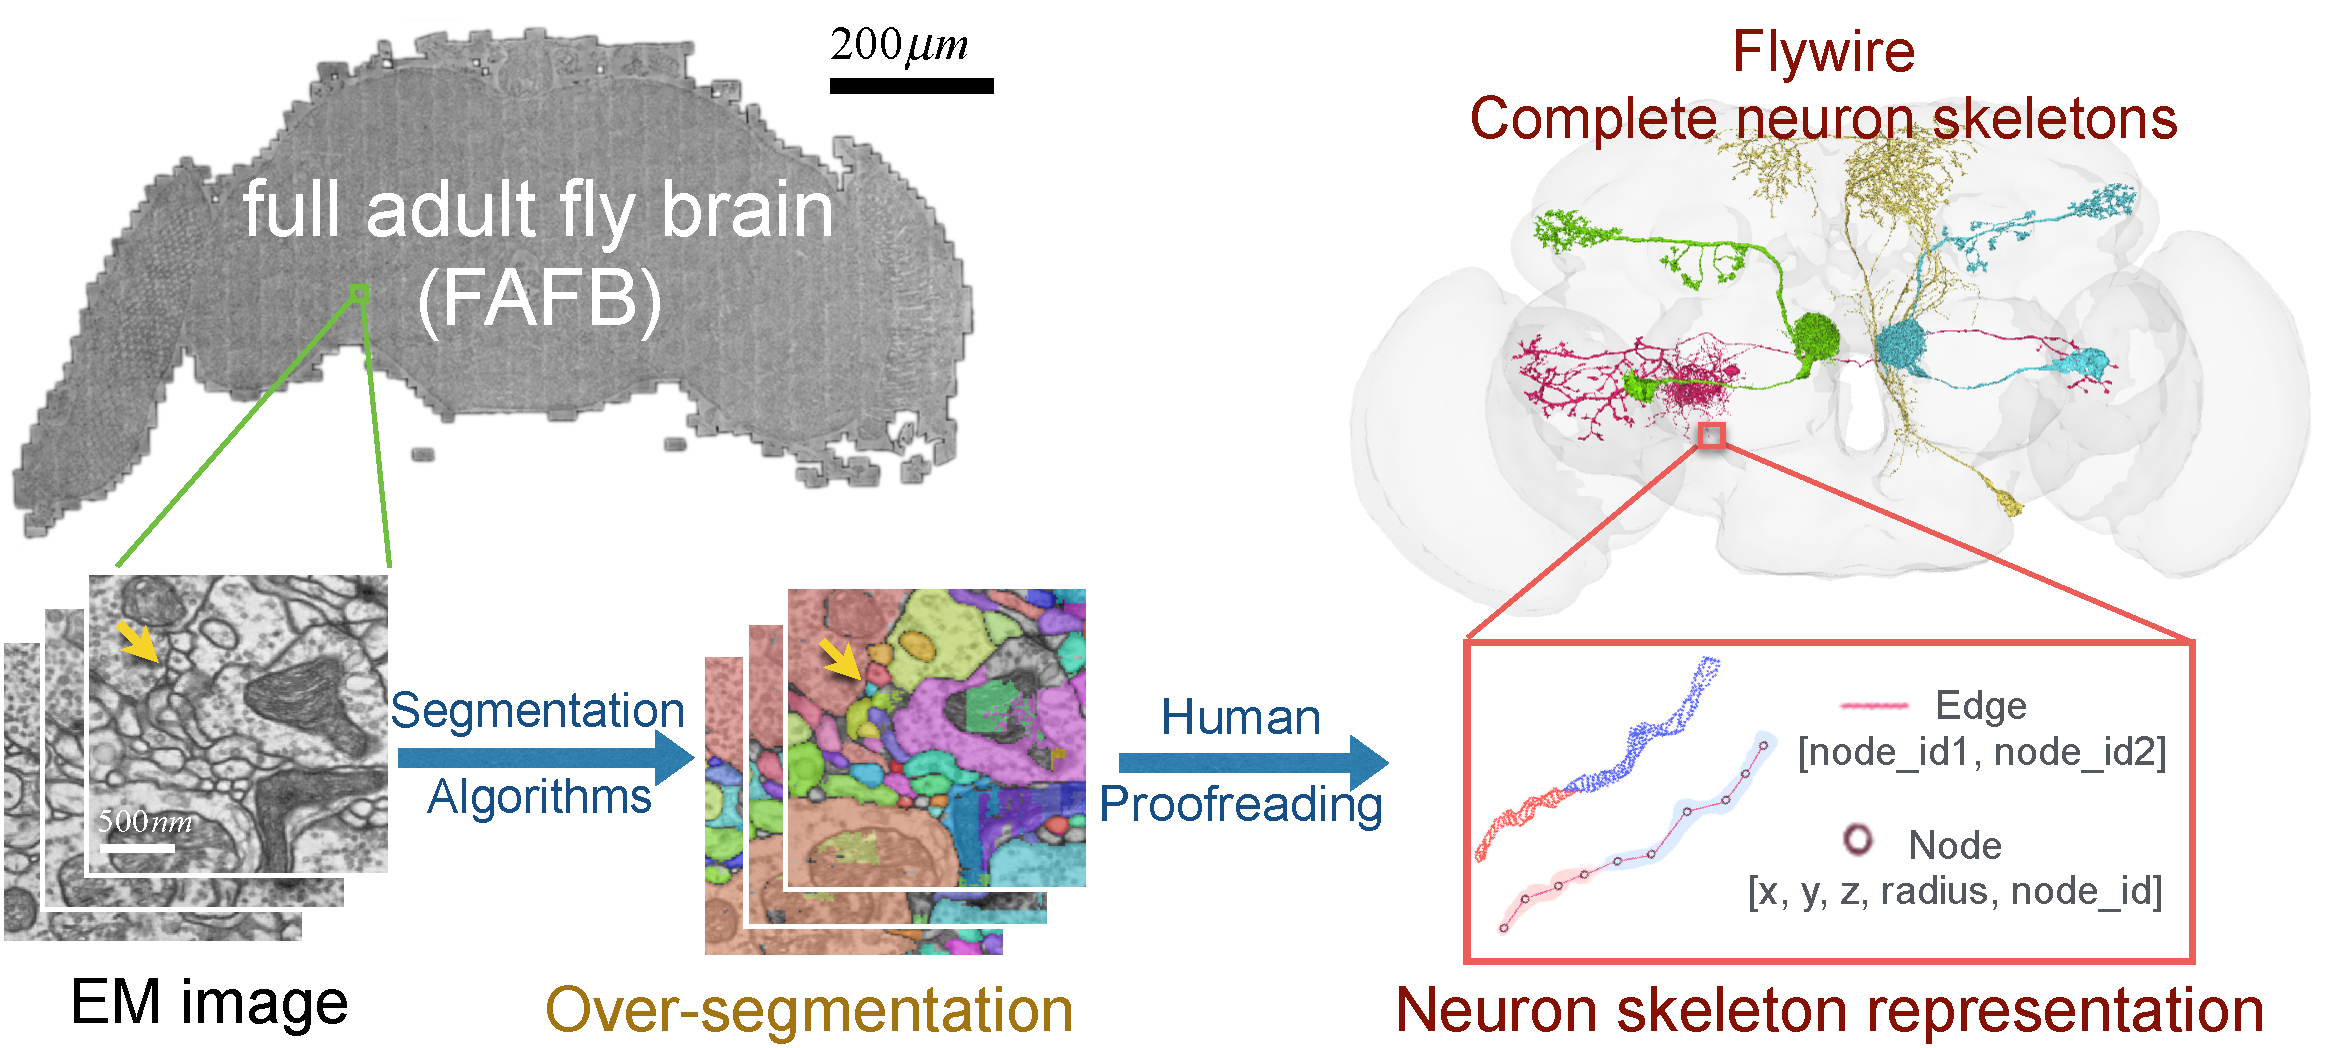
\includegraphics[width=0.48\textwidth]{figs/data-reb.pdf}
    %\vspace{-9pt}
    \caption{The pipeline of large-scale neuron reconstruction consists of EM image over-segmentation and human proofreading for complete neuron reconstruction. Each neuron is represented by a tree-structure skeleton. 
  }
    \label{fig:neuronal-data}
\end{figure}

\begin{figure*}
    \centering
    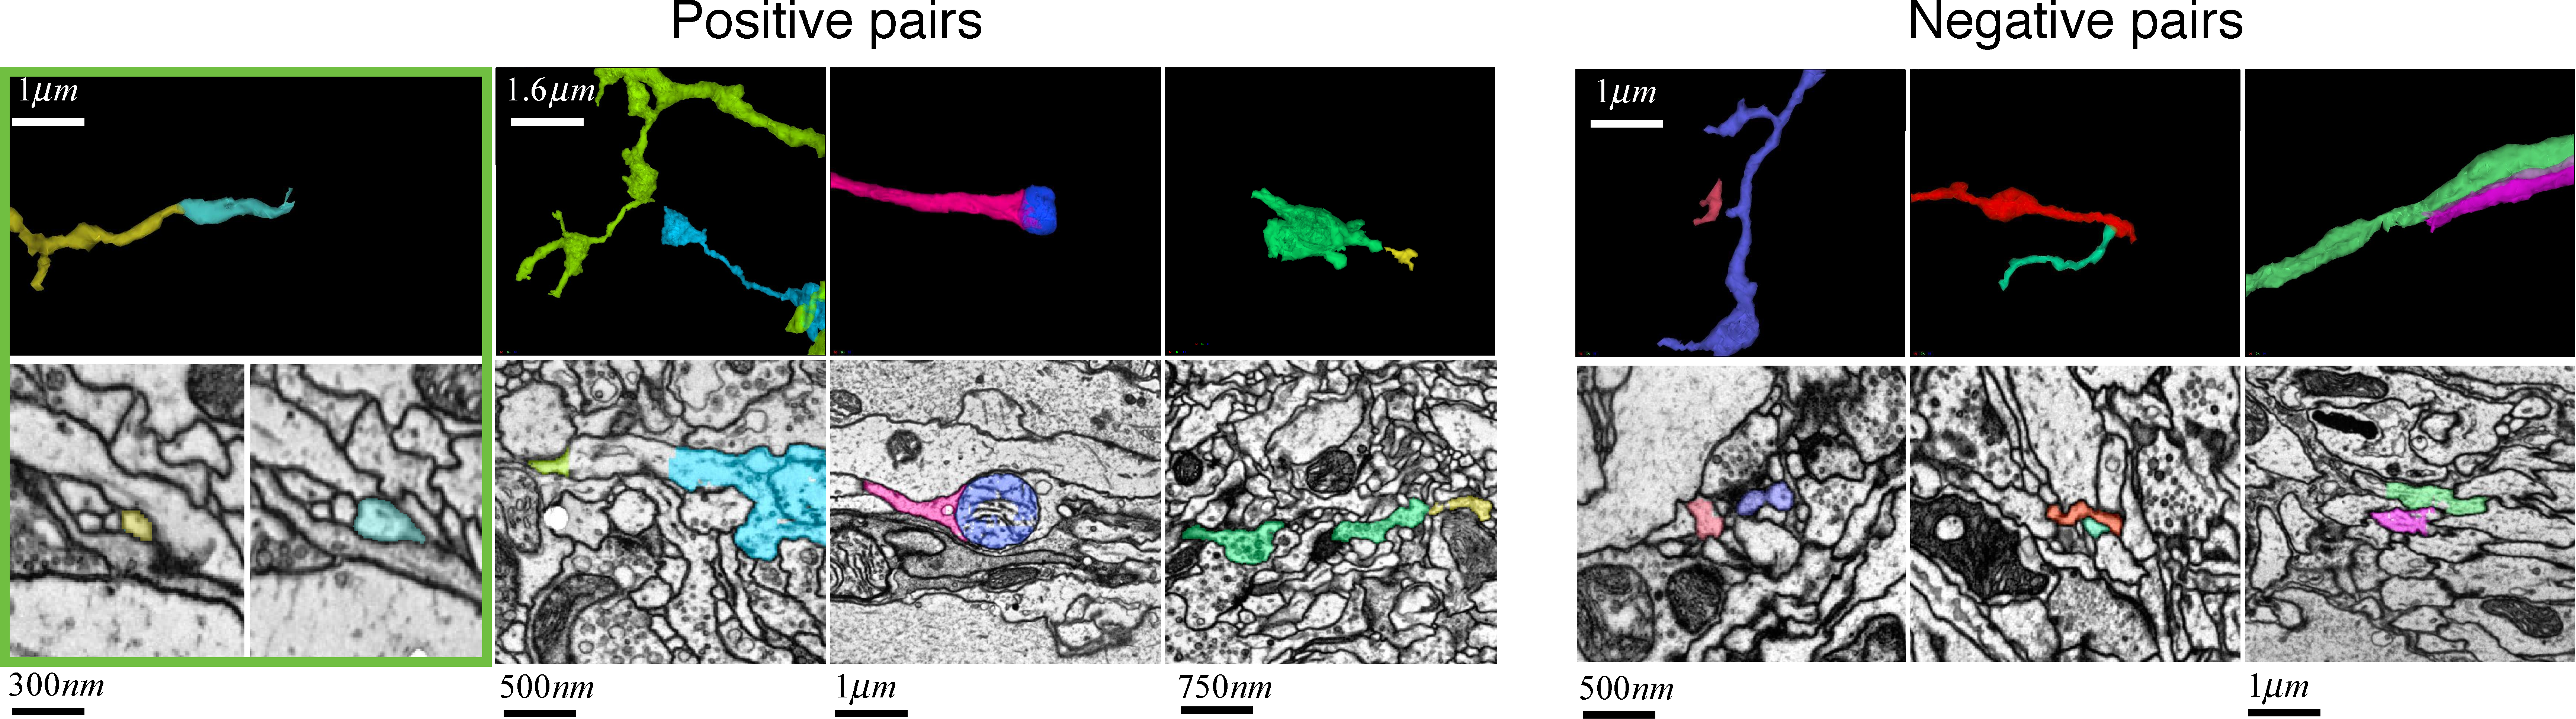
\includegraphics[width=\textwidth]{figs/dataset-main.pdf}
    \caption{Example of sample pairs from FlyTracing. The first row shows their 3D meshes (segment instances denoted by color), with the representative EM image slices shown below. To determine whether two segments belong to the same neuron, human tracers frequently cross-reference their 3D meshes and adjacent EM image slices.}
    \label{dataset}
\end{figure*}